\documentclass[10pt]{article}
\usepackage{icmlko}

\icmlmeta{IP 파운데이션 월드모델}{253}{더 모아도 안 된다}{도서의 여지를 ``수집 문제''로 적은 지 한 사이클 만에 스스로 반증한다 --- 학습을 덜어 내면 오히려 좋아진다}

\begin{document}

\twocolumn[
\icmlheader

\begin{abstract}
노트 252는 도서를 유일한 진짜 여지로 짚고($+$0.177, 몫 6.2\%) 원인을
\textbf{수집}이라고 적었다 --- 학습 80건에 유보 163건으로 학습이 유보보다
적은 유일한 도메인이라서다. \textbf{그 진단이 틀렸다.} 값싼 확인이 있었는데
안 했다: \emph{학습을 덜어 내 보는 것}. 80 $\to$ 60 $\to$ 40 으로 줄이면
도서가 0.3212 $\to$ 0.3347 $\to$ \textbf{0.3604 로 올라간다}. 기울기가
$-$0.019/ln 이다 --- \textbf{도서 제 학습 자료가 도서를 해치고 있다.} 20$\sim$28
건만 남기면 0.3482 로 굳는데, 그 값은 시대를 어떻게 잘라도 똑같이 나온다.
\textbf{풀링으로 되돌아간 값}이고, 지금 판(0.3212)은 그보다 \emph{아래}다.
가는 김에 제일 그럴듯한 수집안도 닫았다 --- \texttt{book\_records} 396건 중
\textbf{153건이 전자책으로 빠져 있고 그중 58건이 2025년 이전}이라 학습을
80에서 138로 키울 수 있어 보였다. 못 쓴다: 전자책 여부가 라벨과
\textbf{$\rho{=}-0.81$}(학습)이고 판형 · 무게가 전자책 0.0\% 대 종이책
99.6\% 라 결측 무늬가 완벽한 형식 깃발이다. \texttt{sales\_point} 자체가 두
매장의 서로 다른 계수기다. \textbf{노트 35의 제외는 옳았다.} 학습을 최근으로
자르는 것($+$0.041)도 $t{=}1.52$ 에 판 $-$0.0006 이라 채택 못 한다.
\textbf{남는 결론}: 도서의 여지는 양이 아니라 \emph{모집단}의 문제이고,
같은 자리에서 더 모으는 것으로는 못 메운다.
\end{abstract}
]

\section{한 사이클 만에 틀렸다}

노트 252는 프로그램 수준의 결론을 냈다 --- 축 열일곱의 여지가 $+$0.013 뿐이고,
그중 실제로 큰 곳은 도서 하나($+$0.177)이며, 원인은 라벨을 안 보고도 보인다:

\begin{quote}\small
도서는 학습 80건에 유보 163건으로 학습이 유보보다 적은 유일한 도메인이고
$\dots$ 도서의 여지는 모형이 아니라 \textbf{수집}이다.
\end{quote}

그럴듯했고, 표를 보면 정말 그렇게 보인다. 그런데 그 문장은 \textbf{안 재고
쓴 것}이다. 재는 법이 값싼데도 --- 학습을 덜어 내 보면 된다. 자료가 모자라서
못 하는 것이라면 덜어 낼수록 나빠져야 한다.

\section{덜어 내면 좋아진다}

\begin{figure}[t]
\centering
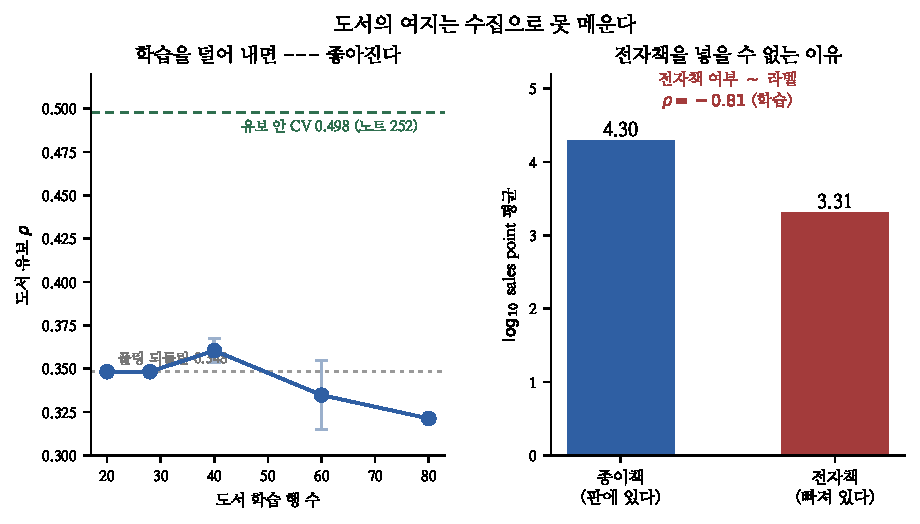
\includegraphics[width=\columnwidth]{figs/book.pdf}
\caption{왼쪽 --- 도서 학습 행을 무작위로 덜어 내며 잰 유보 $\rho$(씨앗 셋).
오른쪽 --- 전자책을 못 넣는 이유.}
\end{figure}

\begin{center}\small
\begin{tabular}{rrrr}
\hline
남긴 학습 & 도서 $\rho$ & SD & 판 \\
\hline
80 (전부) & 0.3212 & --- & 0.4569 \\
60 & 0.3347 & 0.020 & 0.4567 \\
\textbf{40} & \textbf{0.3604} & 0.007 & 0.4549 \\
28 & 0.3482 & 0.000 & 0.4540 \\
20 & 0.3482 & 0.000 & 0.4540 \\
\hline
\end{tabular}
\end{center}

기울기가 $d\rho / d\ln n = \mathbf{-0.019}$ 다. \textbf{도서의 제 학습 자료가
도서를 해친다.}

20$\sim$28건에서 0.3482 로 굳는 것도 말을 한다. 시대를 어떻게 잘라도 --- 2020년
이후만 남겨도, 2015년 \emph{이전}만 남겨도 --- 정확히 0.3482 다. 그 값은
모형이 도서 제 계수를 안 쓰고 \textbf{풀링으로 되돌아간} 값이다(F21의
\texttt{min\_rows}$=$150 이 도서 80건을 이미 걸러내고 있고, 남는 것은 F18
나무다). 그리고 \textbf{지금 판의 도서(0.3212)는 그 되돌림보다 아래}다.

\section{제일 그럴듯한 수집안을 닫았다}

수집이 답이라면 어디서 모으나. \texttt{book\_records.json} 을 열어 보니
\textbf{396건 중 243건만 판에 실려 있었다.} 빠진 153건이 전자책이고,
\textbf{그중 58건이 2025년 이전}이다 --- 넣으면 학습이 80에서 138로 늘고
유보 분모는 안 건드릴 수도 있다. 노트 35가 ``판형 결측이 형식을 누출한다''고
제외해 둔 것인데, 지금 판에는 노트 213 · 214 이후로 그런 누출을 다루는 법이
생겼으니 다시 볼 만했다.

쟀다.

\begin{center}\small
\begin{tabular}{lrr}
\hline
 & 전자책 & 종이책 \\
\hline
건수 & 153 & 243 \\
판형(width) 있음 & \textbf{0.0\%} & 99.6\% \\
무게 있음 & \textbf{0.0\%} & 99.6\% \\
쪽수 · 정가 있음 & 100\% & 99.6\% \\
$\log_{10}$ sales point & 3.31 & 4.30 \\
\hline
\end{tabular}
\end{center}

\[ \rho(\text{전자책 여부},\ \text{라벨}) = -0.811 \ (\text{학습}), \quad
   -0.656 \ (\text{유보}). \]

Mann--Whitney $p = 3\times10^{-39}$ 이다. 결측 무늬(판형 · 무게)가
\textbf{완벽한 형식 깃발}이고 그 깃발이 라벨의 대부분을 설명한다. 넣으면
판이 오르겠지만 모형이 배우는 것은 ``전자책인가''뿐이다. 게다가
\texttt{sales\_point} 는 두 매장의 \emph{다른 계수기}라, 노트 224가 가른
``라벨 두 종류''를 한 도메인 안에서 섞는 셈이다.

\textbf{노트 35의 제외는 옳았다.} 2년 전 결정이 지금 규약으로도 옳다는 것을
확인한 셈이다.

\section{최근으로 자르는 것도 안 된다}

학습이 해롭다면 해로운 부분만 자르면 된다. 도서 학습 80건은 1999--2025에
흩어져 있다(1995--99:1 · 2000--04:13 · 2005--09:4 · 2010--14:12 ·
2015--19:16 · 2020--24:34).

\begin{center}\small
\begin{tabular}{lrrrr}
\hline
도서 학습 & $n$ & 도서 차 & 짝 SE & $t$ \\
\hline
2015 이후만 & 50 & $+$0.0408 & 0.0269 & 1.52 \\
2020 이후만 & 34 & $+$0.0270 & 0.0285 & 0.95 \\
\hline
\end{tabular}
\end{center}

둘 다 잡음 안이고 \textbf{판은 오히려 내려간다}($-$0.0006 · $-$0.0028).
노트 248의 규약대로 도메인 수는 SE 와 함께 읽어야 하는데, 도서 SE 가
0.073 이라 $+$0.04 는 근거가 못 된다. 채택 안 한다.

\section{양이 아니라 모집단이다}

정리하면 도서에 대해 아는 것은 이렇다.

\begin{itemize}
\item 유보 \emph{안}에서 CV 로 배우면 0.498 이 나온다(노트 252). 축이 도서
2025$+$ 를 설명할 힘은 있다.
\item 그런데 도서 \emph{학습}으로 배우면 0.321 이고, 학습을 버리면 0.348 로
오른다. 학습이 가르치는 관계가 유보의 관계와 다르다.
\item 학습을 늘리는 길(전자책)은 라벨이 달라 막혀 있다.
\item 학습을 최근으로 좁히는 길은 잡음 안이다.
\end{itemize}

\textbf{양의 문제가 아니라 모집단의 문제다.} 도서 레코드는 베스트셀러 목록
스크랩이라 2026년이 209건 · 2025년이 49건인데 2010년대는 다 합쳐 30건 남짓이다.
``2020년 이전 베스트셀러''는 ``지금 잘 팔리는 옛 책''이고, ``2026년
베스트셀러''는 ``지금 잘 팔리는 새 책''이다. 이름만 같은 두 모집단이다.
노트 209가 라벨의 누적성을 지적한 것과 같은 병의 다른 얼굴이다.

노트 252의 마지막 줄 --- ``다음 이득은 새 정보에서 온다'' --- 은 살아남는다.
다만 \textbf{``새 정보''가 ``같은 자리에서 더''는 아니라는 단서}가 붙는다.

\paragraph{남은 것}
\begin{center}\small
\begin{tabular}{ll}
\hline
갈래 & 왜 \\
\hline
도서 학습이 해롭다 & 판에서 빼면? 되돌림 0.348 $>$ 지금 0.321 \\
같은 검사 아홉 곳 & 다른 도메인도 제 학습이 해로운가 \\
웹툰 $+$0.051 & 몫 27\%. 도서보다 판에 크다 \\
고정 창 라벨 & 노트 209의 숙제. 모집단 문제의 뿌리 \\
\hline
\end{tabular}
\end{center}

\paragraph{규약} ``자료가 모자라서''라고 쓰기 전에 \textbf{덜어 내 본다.}
덜어서 안 나빠지면 모자란 게 아니다. 한 줄짜리 실험이고, 이번에 그것을
안 해서 노트 하나를 틀리게 썼다.

\end{document}
